\chapter{Future Work}
\label{Cha:Future_Work}
This chapter list the aspect of Cisco system and Indoor location based service work, for future semesters.

\begin{itemize}
	\item Research better ways of obfuscating the MAC addresses so it is not stored in plain text.
	\item Secure the connection between Cisco system and the DB server, so data is not possible to sniff.
\end{itemize}


\section{Data Flow from Cisco to the Database}\label{sec:data_flow}
\begin{figure}[ht]
	\begin{center}
		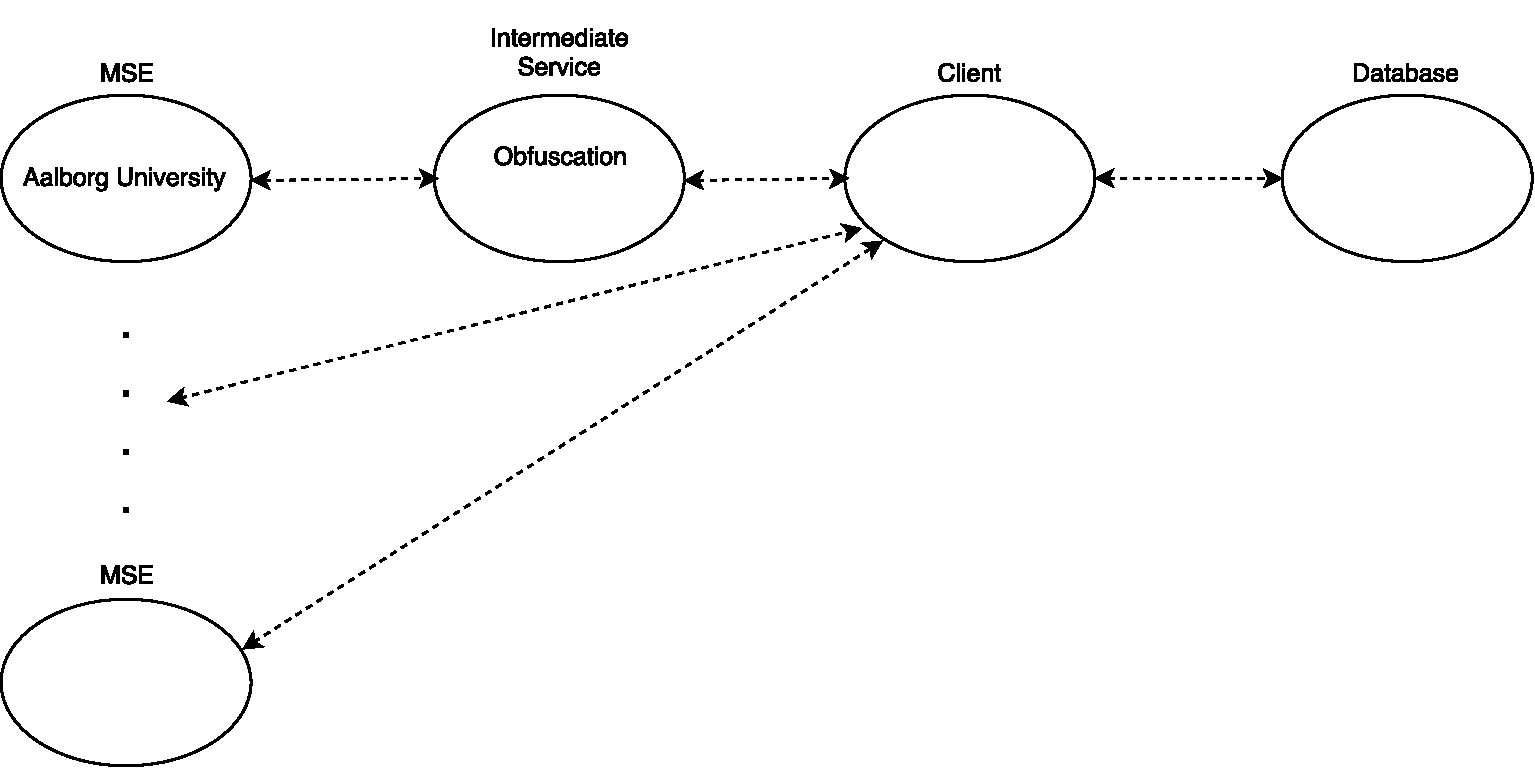
\includegraphics[scale=0.7]{graphics/ciscoNew.pdf}
		\caption{Cisco systems}
		\label{fig:cisco_systems}
	\end{center} 
\end{figure}
\Cref{fig:cisco_systems} shows how the information flow is intended. The client connecting to the Cisco services can function as a server that requests data from all Cisco services that we have access to. Alternatively, a server can be implemented for each Cisco service. However, this solution has several downsides. First, it means corporations supplying the aSTEP project with information will have to have hardware running the server, which requires maintenance. Second, this solution is not scalable. The server running the aSTEP database will potentially be overloaded, as it has to handle each individual Cisco system sending information. As more Cisco systems are added, there will be less time to process received data. An alternative approach is to have the aSTEP database server request data from the mobile apps, however, with an increase in connected Cisco systems, the interval at which we receive new information from a given system also increases. The optimal solution to this issue is to create a hierarchy of servers, such that the database server only receives data from a constant amount of intermediate servers, each of which also receive information from an amount of sources. During the start up of the aSTEP project we have access to a single Cisco MSE system, and as such we will not focus on building this hierarchy. However, as the project grows and additional Cisco systems are integrated, it will eventually become a necessity.

\section{The Future of Our IPS}\label{sec:futureSystem}
As described in \cref{sec:ourSys} we have been working on building our own IPS. However, it was not possible for us to finish it as we encountered a significant difficulty. The obstacle we encountered was not being able to acquire the RSSI, and thus making it impossible for us to make further meaningful progress on our system within the remaining time limit. We do however believe it would be a fitting and interesting task for future developers.

The first step, if someone is to furtherer develop the system, should be to acquire the RSSI for devices connected to the network. The next step should be to expand the range of attainable devices by allowing multiple access points. From there is should be possible to calculate the distance between each access point based on the signal strength. This calculation can be performed by utilising one of the methods described in \cref{sec:tracking_approach}. By implementing these features it would be possible to calculate the positions of devices on the network, which we believe would be a crucial component of creating the system.

If the described features were implemented, a set of secondary functionality could be considered. The system could be expanded to receive the signal strength for all devices within the networks perimeter, connected or not. This would allow the system to track everyone within its coverage and thereby give it a more accurate view of the area.
Another beneficial feature the system could support, is be to calculate an estimate of how likely it is that the found locations are correct. This estimate could be similar to that the MSE provides with its \textit{confidenceFactor} described in \cref{sec:class_design}. This estimate will be useful for comparing the system's precision with other systems as descried in \cref{sec:ourSys}. 

\section{Coordinate Formats}
As described in \cref{sec:geo_coordinates}, there are three formats for geographical coordinates. We have chosen to provide the decimal degree format because it is the format used by the outdoor location groups and the format requested by the application group utilising indoor positioning.
However, future applications as well as future development on existing applications may need other formats. We have in \cref{sec:geo_coordinates} provided the necessary calculations to change the format. These calculations can be used in the future to implement the api.
